\chapter{Introdução}

% \todo[inline]{Adicionar um parágrafo para explicar o que é HPC.}

Nos primeiros computadores, avanços tecnológicos possibilitavam aumentar o
desempenho de semicondutores e das arquiteturas por meio do aumento da
frequência. Contudo, com o aumento da frequência, ocorre um maior consumo de
energia e, consequentemente, a temperatura do \textit{chip} aumenta. Desta
forma, indústrias começaram a investir em outros meios para aumentar o
desempenho de arquiteturas, um exemplo, são os processadores \textit{manycore}.

Arquiteturas \hpc são exemplos de \textit{manycores} utilizadas para o
processamento de uma imensa quantidade de dados ou para aplicações que precisam
de um grande quantidade de tempo para serem executadas. Supercomputadores e
\textit{clusters} de computadores são utilizados para tornar a computação de
aplicações ou dados tratável do ponto de vista computacional. Essas arquiteturas
são utilizadas em aplicações científicas ou, mais atualmente, em áreas de Banco
de Dados, devido à problemas com \textit{Big Data}. Normalmente, arquiteturas
\hpc são compostas por uma \cpu{} e aceleradores (e.g, \gpu).

Atualmente, os \textit{cores} (núcleos) de arquiteturas \textit{manycore}
aumentam continuamente. A Figura~\ref{fig:graphCores} mostra o número de
\textit{cores} e energia consumida pelo supercomputador em primeiro lugar no
\textit{ranking} do TOP500, confirmando esse comportamento. Pode-se perceber o
aumento significativo da quantidade de \textit{cores} ao longo dos anos.
% \todo[inline]{Adicionar comentário sobre imagem de \textit{cores}}
Além disso, pode-se verificar o consumo de energia que aumenta de acordo com o
número de \textit{cores} utilizados pelo supercomputador. Chegando à um total,
atualmente, de $15$ kW/h.

% \todo[inline]{Explicar que há uma tendência no crescimento de núcleos em arquiteturas de HPC para se conseguir processar mais dados em menos tempo. Adicionar a figura do TOP 500. Essas arquiteturas são compostas normalmente por CPUs (multicore) e aceleradores (ex. GPUS).}



Até a última década, o desempenho das arquiteturas \hpc era quantificado quase
que exclusivamente pelo seu poder de processamento, usualmente medido por
\flops. Contudo, o consumo excessivo de energia é uma barreira para o aumento de
dsempenho de forma escalável nestas plataformas.

% \todo[inline]{Ressaltar o relatório DARPA/IPTO e falar da eficiência energética do supercomputador nro 1 e quão distante ele está do ideal.}

Essa preocupação com o aumento de energia é ressaltada pelo relatório emitido
pelo Departamento de Defesa do Governo dos Estados Unidos (DARPA/IPTO)
~\cite{Kogge2008}. O relatório ressalta que para atingir o
\textit{Exascale}(10$^{18}$) é necessário, aproximadamente, 20 MW, isto é, com
essas características, um supercomputador deve ser capaz de efetuar 50 GFlops/W.
Por outro lado, atualmente, os supercomputadores mais energicamente eficientes
possuem uma eficiência energética inferior à $6,1$ TFlops/W, com um pico
inferior à $8,2$ TFlops/W. Esse valor é 8 vezes menor que o ressaltado pelo
relatório da DARPA/IPTO, sendo assim, atualmente a eficiência energética de
supercomputadores está bem distante da ideal. Portanto, para que
supercomputadores tenham potencial para atingir o \textit{Exascale} é necessário
um consumo energético viável e um alto desempenho. Contudo, o crescimento dessas
duas variáveis não é proporcional.


Por essa razão, o estudo de técnicas que melhorem a eficiência energética em
plataformas \hpc está se tornando muito importante.  Recentemente, uma nova
classe de processadores \textit{manycore} de baixa potência tais como o Sunway
SW26010~\cite{sunway:2016}, Mellanox TILE-Gx~\cite{Valero:2012} e Kalray
\mppa~\cite{Castro-IA3:2013} foram desenvolvidos. Esses processadores possuem
centenas de núcleos de processamento capazes de lidar com paralelismo de dados e
tarefas com baixo consumo de energia.

Apesar desses processadores \textit{manycore} fornecerem uma melhor eficiência
energética~\cite{Castro-IA3-JPDC:2014}, eles possuem uma arquitetura particular
que torna o desenvolvimento de aplicações paralelas uma tarefa
desafiadora~\cite{Varghese14,Castro-PARCO:2016,Castro-SBAC-PAD:2014}. Núcleos de
processamento sem coerência de \textit{cache} são, geralmente, distribuídos em
uma arquitetura organizada em \textit{clusters}, onde cada \textit{cluster}
possui uma memória local (compartilhada somente entre os núcleos do
\textit{cluster}). Dessa forma, a comunicação entre \textit{clusters} deve que
ser efetuada através de uma \noc de maneira distribuída.
Por essa razão, o tempo de comunicação pode variar entre os núcleos que estão se
comunicando.
%Explicar as dificuldades.

O \mppa possui 256 núcleos distribuídos em 16 \textit{clusters}, denominados de
\pe, e 4 subsistemas de \io. O ambiente do \mppa é heterogêneo, sendo utilizado
entre os \textit{clusters} e \io, uma comunicação via troca de mensagens, e
dentro de cada \textit{cluster} são utilizados comunicações diretas entre
\pe{}s, por meio de memória compartilhada. As principais dificuldades do
desenvolvimento de aplicações para o \mppa são: \textbf{(i) modelo de
    programação híbrido:} problema citado anteriormente, onde \textit{threads}
em um mesmo \textit{cluster} se comunicam através de memória compartilhada
local, porém a comunicação entre \textit{clusters} é feita explicitamente via
NoC, seguindo um modelo de computação distribuída; \textbf{(ii) comunicação:} é
necessária a utilização de uma \textit{Application Programming Interface} (API)
específica para a comunicação via NoC, similar ao POSIX de baixo nível para
\ipc; \textbf{(iii) memória:} cada \textit{cluster} possui apenas 2MB de memória
local de baixa latência, portanto aplicações reais precisam constantemente
realizar comunicações com o subsistema de E/S e \textbf{(iv) coerência em
    cache:} cada PE possui uma memória \textit{cache} privada e sem coerência
com as \textit{caches} dos demais PEs, sendo necessário atualizar a
\textit{cache} manualmente.

Uma possível solução para os problemas apresentados é a utilização de padrões
paralelos ou \textit{skeletons}~\cite{cole-skeleton:2004}. \textit{Skeletons}
são modelos de programação paralelas em alto nível. Esses modelos fornecem
vantagens para o desenvolvedor, escondendo a complexidade de aplicações
paralelas e distribuídas. Os \textit{Skeletons} especificam, mais precisamente,
os padrões de acesso de dados e comunicação. Desta forma, eles possibilitam aos
desenvolvedores focarem apenas nos algoritmos, ao invés da comunicação,
sincronização de tarefas e escalonamento, que são gerenciados de forma
transparente pelo \fw que implementa um \textit{skeleton}.

Entre os diversos \textit{skeletons} existentes (\textit{map}, \textit{reduce},
\textit{pipeline} e \textit{scan}), o padrão \textit{stencil} é o mais
utilizado em ambientes importantes, como física quântica, previsão do tempo e
processamento de imagens~\cite{gonzalez06,holewinski12}.

%Explicar Stencil? Imagens?

\Fws são utilizados para fornecer uma abstração sobre partes de código que serão
reusadas diversas vezes. Esse \fw pode ser estendido ou adaptado para fornecer
suporte para outras aplicações com diferentes características. Dessa forma, a
utilização de um \fw pode facilitar o desenvolvimento de aplicações para
ambientes onerosos, como ambientes \textit{manycore}.

Muitos \fws foram propostos para o auxílio no desenvolvimento de
\textit{stencil} paralelos em ambientes \textit{multicore} e \gpu como o
PSkel~\cite{pereira15}, SkePU~\cite{enmyren10} e SkelCL~\cite{steuwer11}. Em
particular, o PSkel é um \fw que fornece uma abstração em alto nível para o
desenvolvimento em ambientes heterogêneos CPU-GPU, enquanto particiona tarefas e
dados de forma transparente entre CPU e GPU.
%\section{Motivação}

\section{Objetivo}
\subsection{Objetivo Geral}
O objetivo deste TCC é adaptar o \fw ~\pskel para o processador \mppa,
fornecendo as vantagens provenientes do \fw, como a transparência e alta
abstração, para o \mppa. Além de uma portabilidade total de aplicações já
desenvolvidas para o \fw.

\subsection{Objetivos Específicos}
\begin{itemize}
	\item Efetuar a comunicação de tarefas de forma transparente.
    \item Utilizar a \noc para a comunicação entre \io e \textit{clusters}.
    \item Aplicações executadas no \fw não serão alteradas para execuções feitas
        no \mppa.
    \item As técnicas utilizadas para a comunicação devem considerar o limite de
        memória de cada \textit{cluster}.
\end{itemize}

\section{Organização do Texto}
........

% Introduzir Figura
%\begin{figure}
%	   \centering
%	   		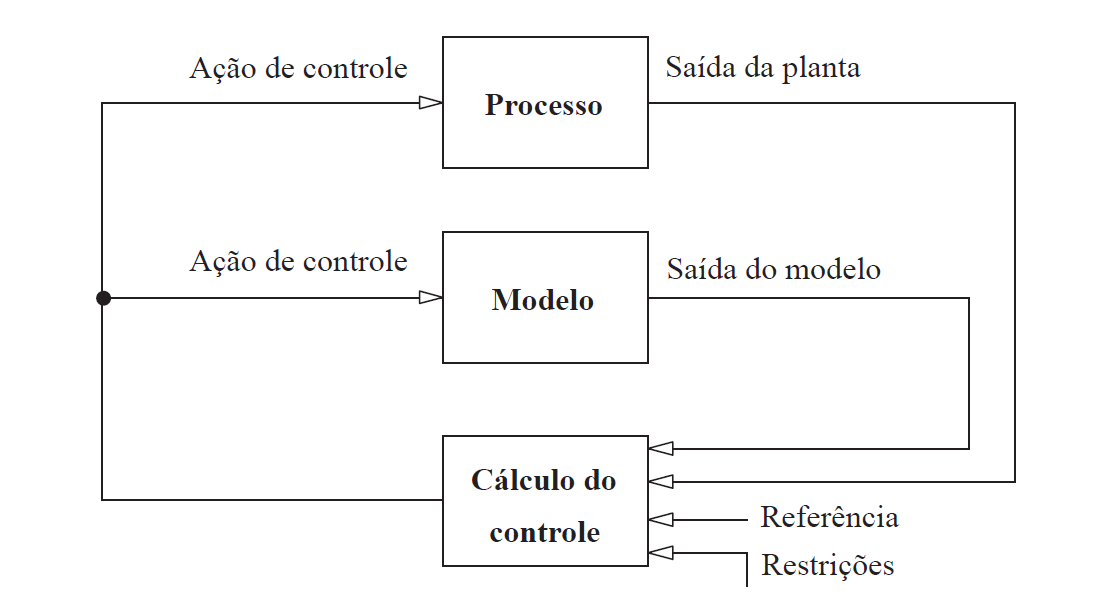
\includegraphics[scale=0.35]{figs/MPCbase.PNG}
%	   \caption{Algoritmo MPC}
%	   \label{label para referencia cruzada Figura}
%\end{figure}


% Lista de Item

%\begin{itemize}
%	\item item 1
%	\item item 2
%	\item item 3
%\end{itemize}

% Equação
%\begin{equation}
%	\label{label para referencia cruzada %equacoes}
%	y(t)=\sum_{i=1}^{\infty}h_i\Delta u(t-i)
%\end{equation}

% Equação em linha
%$\hat{y}(t+k\mid t)= \sum^\infty_{i=1} g_i %\Delta u(t+k-i\mid t)$

% Citação -  Criei o arquivo de bibliografia usando o jabref

%\cite{Camacho2007}

% Referencia Cruzada de Figura
%\ref{label para referencia cruzada Figura}

% Referencia Cruzada de Equação
%\ref{label para referencia cruzada equacoes}


% Tabelas

%\begin{table}[h]
%\begin{center}
%     \caption{Índices 1 para casos factíveis}
%     \begin{tabular}{| l | l | l | l |}
%     \hline Índice & LP Petro & LP 2 & %Diferença\\
%     \hline $SES_y$& 60.5406 & 60.5492 & %-0.0087\\
%     \hline $SES_u$& 1166.1464 & 1166.1464 & 2.36*$10^{-9}$ \\
%     \hline

%    \end{tabular}
%\label{table:indices1}
%\end{center}
%\end{table}
